% ! TeX root = thesis_en.tex

\chapter{User documentation}
\label{ch:user}

Both the changes in the Clang-Tidy infrastructure and our new checker focuses heavily on LLVM's Clang-Tidy.
Clang-Tidy is a Clang-based \CC{} ``linter'' tool. Its purpose is to provide an extensible framework for diagnosing and fixing
typical programming errors, like style violations, interface misuse, or bugs that can be deduced via static analysis.
Clang-Tidy is modular and provides a convenient interface for writing new checks. % http://clang.llvm.org/extra/clang-tidy/

The tool, after upstreaming, will be found in the LLVM project repository at \url{http://github.com/llvm/llvm-project}.

\section{Install guide}

\subsection{System Requirements}

Table 2.1 shows the system requirements and supported compilers for building
LLVM. The checkers were developed with Ubuntu 20.04 and tested on Ubuntu 18.04, and WSL Ubuntu 20.04.

Building and using LLVM's Clang-Tidy takes a lot of time on weaker computers. The minimum recommended memory size
for building is 16 GiB, and the optimal amount is 64 GiB of memory. % continue with the recommendation  

\begin{table}[H]
	\centering
	\begin{tabular}{ | m{0.33\textwidth} | m{0.33\textwidth} | m{0.33\textwidth} | }
		\hline
		\textbf{Operating system} & \textbf{Processor architecture} & \textbf{Compiler} \\
		\hline \hline
		Linux & x861 & gcc, clang \\
		\hline
		Linux & amd64 & gcc, clang \\
		\hline
		Linux & arm & gcc, clang \\
		\hline
		Linux & Mips & gcc, clang \\
		\hline
		Linux & PowerPC & gcc, clang \\
		\hline
		Solaris & V9 & gcc \\
		\hline
		FreeBSD & x861 & gcc, clang \\
		\hline
		FreeBSD & amd64 & gcc, clang \\
		\hline
		NetBSD & x861 & gcc, clang \\
		\hline
		NetBSD & amd64 & gcc, clang \\
		\hline
		macOS2 & PowerPC & gcc \\
		\hline
		macOS & x86 & gcc, clang \\
		\hline
		Cygwin & x86 & gcc \\
		\hline
		Windows & x86 & Visual Studio \\
		\hline
		Windows64 & x86-64 & Visual Studio \\
		\hline
	\end{tabular}
	\caption{System requirements and supported compilers for building LLVM.}
	\label{tab:clang-req}
\end{table}

Software requirements include (at least) GCC version \emph{7.1.0}, CMake version \emph{3.13.4}, Python version \emph{3.6} and GNU Make version \emph{3.79}.

\subsection{Building from source}

These commands will compile LLVM from source. The building process with parameters can be found on the \texttt{README.md} of
LLVM project Github repository,\footnote{\url{http://github.com/llvm/llvm-project\#readme} accessed 2022. 05. 03.} or the Getting
Started\footnote{\url{http://clang.llvm.org/get_started.html}, accessed 2022. 05. 03.} page of Clang documentation. The commands I used for
the compilation are shown in \cref{lst:compile-commands}.

\begin{listing}
	\begin{minted}{Bash}
	git clone http://github.com/llvm/llvm-project.git
	cd llvm-project
	mkdir Build

	# cmake -S llvm -B build -G <generator> [options]
	cd Build/
	cmake \
		-DCMAKE_EXPORT_COMPILE_COMMANDS=ON \
		-DLLVM_ENABLE_PROJECTS="llvm;clang;clang-tools-extra" \
		-DLLVM_TARGETS_TO_BUILD="X86" \
		-DLLVM_APPEND_VC_REV=OFF \
		-DLLVM_ENABLE_BINDINGS=OFF \
		-DLLVM_USE_RELATIVE_PATHS_IN_FILES=OFF \
		-DBUILD_SHARED_LIBS=ON \
		-DLLVM_USE_LINKER="lld" \
		-DLLVM_PARALLEL_LINK_JOBS=3 \
		-DCMAKE_BUILD_TYPE=Release \
		-DLLVM_ENABLE_DUMP=ON \
		-DLLVM_ENABLE_ASSERTIONS=ON \
		-G Ninja \
		../llvm

	# cmake --build build [-- [options] <target>] or your build system specified above directly.
	ninja -j12 clang-tidy llvm-symbolizer
\end{minted}
	\caption{Compiling LLVM from source on a weaker machine.}\label{lst:compile-commands}
\end{listing}

Explanation for some flags: at \mintinline{Bash}{LLVM_USE_LINKER} we can change the linker we are using, either Gold or LLD (Linker for LLVM). The
latter needs to be installed. \mintinline{Bash}{LLVM_PARALLEL_LINK_JOBS} and \texttt{-j} at Ninja sets the CPU multiprocessing job capacity. The recommended amount for
\mintinline{Bash}{LLVM_PARALLEL_LINK_JOBS} is one quarter of the amount of cores available, and full Ninja job amount should be $cores - 2$. I used these commands on a
server with 32 GiB memory and 14 (virtual) CPU cores.


\section{Running by Translation Units}
\label{by-TU}

The user can give Clang-Tidy multiple translation units to run on, and it will emit diagnostics separately for each one. You run it by
using \mintinline{Bash}{clang-tidy -checks='-*,misc-discarded-return-value' -p ./Build a/main.cpp b/main.cpp},
where the ``checks'' first disables all checkers with \mintinline{Bash}{-*}, then enables our checker, the \texttt{-p} flag gets the build path that reads a
compile command database, and finally we give the paths to the paths of our source files~\cite{flags}. Here we are getting two separate diagnostics
for our two separate files or translation units.

\begin{listing}[H]
	\begin{minted}{Bash}
	bahramib@cc:~/MyFolder/TestFolder$ clang-tidy -checks='-*,misc-discarded-return-value' -p ./Build a/main.cpp b/main.cpp

	/home/bahramib/MyFolder/TestFolder/a/main.cpp:12:9:
		warning: return value of 'maybe_check_this' is used
		in most calls, but not in this one [misc-discarded-return-value]

			MyClass::maybe_check_this();
			^

	/home/bahramib/MyFolder/TestFolder/a/main.cpp:12:9: note:
		value consumed or checked in 75% (3 out of 4) of cases
	\end{minted}
\caption{Diagnostic output without project-level knowledge.}
\end{listing}



\begin{figure}[H]
	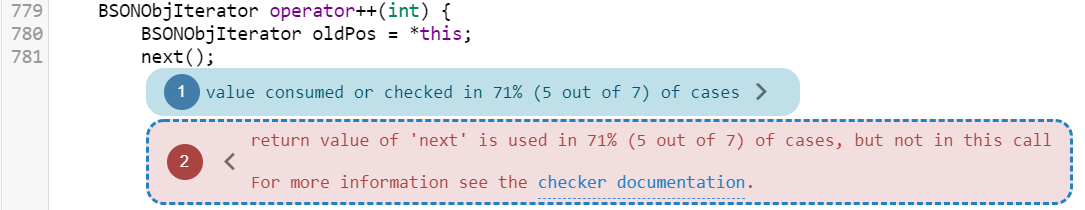
\includegraphics[width=\linewidth]{images/codechecker_first_ss_mongo_single_50.png}
	\caption{A report of the diagnostics of MongoDB's source on CodeChecker with 50\% threshold on a single TU.}
	\label{fig:mongo50single}
\end{figure}

Clang-Tidy is supported by CodeChecker.~\cite{codechecker}

\subsection{Configuring the threshold}

As previously discussed, the ratio of the amount of checked function calls and all the function calls is very important for the
diagnosis, since we do not necessarily want to be notified of all the unused calls, but let us say if a function's return value
is used in at least 65\% of all calls, we might want to be warned about the missing unchecked 35\%.

The checker has an option for this called the \texttt{ConsumeThreshold}, that is the percentage above which we would like to be warned,
but not under.
You can configure \texttt{ConsumeThreshold}, and any Clang-Tidy checker option with Tidy's \mintinline{text}{-config} flag. Here you will have to type
the name of the checker and its option member, with the desired value as a \emph{key-value pair}. This is how it looks with 50\%:
\mintinline{text}{-config='{CheckOptions: [{key: misc-discarded-return-value.ConsumeThreshold, value: 50}]}'}. With this option the full
command looks like this:
\mintinline{text}{clang-tidy -checks='-*,misc-discarded-return-value'-config='{CheckOptions: [{key: misc-discarded-return-value.ConsumeThreshold, value: 50}]}' -p ./Build a/main.cpp b/main.cpp}.

\subsection{Supressing Warnings}

Let us review what is wrong with our code in \cref{unsuppressed}. In function \texttt{foo}, we forget to use our parameter \texttt{p}, and we do not
check the return value when calling \texttt{foo}. These triggers one warning for each mistake as seen in \cref{fig:compiler-warning}.

\begin{listing}[H]
\begin{minted}{CPP}
[[nodiscard]] int foo(int p) {
  return 1;
}
int main(int argc, char**) {
  foo(argc);
}
\end{minted}
\caption{An example of both unused parameter and ignored return value with nodiscard.}\label{unsuppressed}
\end{listing}

\begin{figure}[H]
	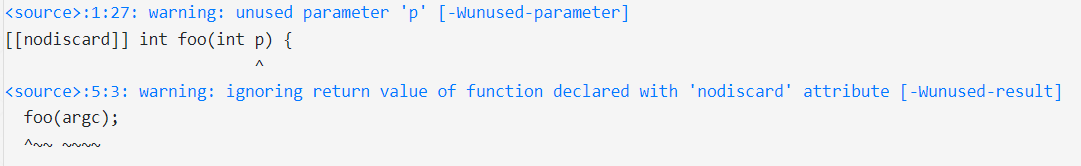
\includegraphics[width=\linewidth]{images/nodiscard_warning.png}
	\caption{The compiler warnings.}
	\label{fig:compiler-warning}
\end{figure}

If we do not want to fix these issues, but rather silence our warnings, we can simply write \mintinline{CPP}{(void)} before the call
to cast it to \mintinline{CPP}{void} and trick the compiler into thinking that we did check the return value.
Similarly, we could cast our parameter \texttt{p} to \mintinline{CPP}{void} as a distinct statement to make it seem like we used it. On \cref{suppressed}
we can see the suppressed version that does not yield warnings.

\begin{listing}[H]
\begin{minted}{CPP}
[[nodiscard]] int foo(int p) {
  (void)p;
  return 1;
}
int main(int argc, char**) {
 (void)foo(argc);
}
\end{minted}
\caption{The same example, now with suppressed warnings.}\label{suppressed}
\end{listing}

The suppression of our new checker warnings follows the exact same convention. Casting to \mintinline{CPP}{void} acts as usage of the return
value and thus will not give warnings, despite not actually checking it.

Both the philosophy and practice of silencing a single case of an unchecked function call is essentially the same as silencing the
warning of \mintinline{CPP}{[[nodiscard]]} or an unused parameter. By simply writing \mintinline{CPP}{(void)} before the call, to cast it to void,
tricking the compiler and the checker into thinking it is used, but not affecting anything in reality.
If we got a warning on the line \mintinline{CPP}{foo();}, from the checker or \mintinline{CPP}{[[nodiscard]]}, we will get neither if we change it
to \mintinline{CPP}{(void)foo();}.

\section{Multiple Phase Version}

The updated infrastructure contains two new flags for running Clang-Tidy, \texttt{multipass-phase} and \texttt{multipass-dir}.
\texttt{multipass-phase} is an \mintinline{CPP}{enum} flag, that has three values, \mintinline{CPP}{"collect"}, \mintinline{CPP}{"compact"} and \mintinline{CPP}{"diagnose"}
with the latter as default.
\texttt{multipass-dir} needs a path to a directory where the checkers that support the collect feature can dump their collection data
that they are going to compact and use later.


\subsection{Collect}

The Collect phase, as the name suggest, will have the checkers collect data on each translation unit and write them into unique YAML
files to later reuse this data. This is how you normally run collect phase on the desired files:

\begin{listing}[H]
	\begin{minted}{Bash}
	clang-tidy \
	-checks='-*,misc-discarded-return-value' \
	--multipass-phase=collect \
	--multipass-dir='MyCollectionDirectory' \
	-p ./Build \
	a/main.cpp b/main.cpp
	\end{minted}
\end{listing}

What the Discarded Return Value checker does in this phase is count the amount the declared non-void functions were called,
and count the amount that these function's return values were checked. After finishing counting in one translation unit, it writes the
collected numbers and function names into a YAML file.

After collecting, you do not get any diagnostics or output text, but the desired amount of (in this case 2) YAML files are generated.

\begin{listing}[H]
	\begin{minted}{Bash}
bahramib@cc:~/MyFolder/TestFolder/MyCollectionDirectory$ ls -l
-rw-r--r-- 1 bahramib 196 Apr 30 13:00 misc-discarded-return-value.main.cpp.12949585208029997868.yaml
-rw-r--r-- 1 bahramib 196 Apr 30 13:00 misc-discarded-return-value.main.cpp.4924802982073527590.yaml
	\end{minted}
	\caption{The YAML files containing the collection data.}
\end{listing}

\begin{listing}[H]
	\begin{minted}{YAML}
	# First TU, a/main.cpp
	---
	- ID:              'c:@S@MyClass@F@check_that#S'
	  Consumed:        3
	  Total:           3
	- ID:              'c:@S@MyClass@F@maybe_check_this#S'
	  Consumed:        0
	  Total:           3
	...
	\end{minted}

	\begin{minted}{YAML}
	# Second TU, b/main.cpp
	---
	- ID:              'c:@S@MyClass@F@check_that#S'
	  Consumed:        1
	  Total:           3
	- ID:              'c:@S@MyClass@F@maybe_check_this#S'
	  Consumed:        3
	  Total:           4
	...
	\end{minted}
	\caption{Contents of the results of collecting data.}
\end{listing}

\subsection{Compact}

The Compact phase will iterate through the collected data per checker and have the checkers read, use and compact all the data collected
into one YAML file. Flags aside from \texttt{checks}, \texttt{multipass-phase} and \texttt{multipass-dir} have no effect.

\begin{listing}[H]
	\begin{minted}{Bash}
	clang-tidy \
	-checks='-*,misc-discarded-return-value' \
	--multipass-phase=compact \
	--multipass-dir='MyCollectionDirectory' \
	\end{minted}
\end{listing}

This checker reads the data on each function back and constructs new data similar to the previous ones. If one function is called in multiple
translation units, then it adds the numbers from the TU's YAML file to the new structure. After it is finished, the data is
written into a single YAML file.

This phase does not write anything on standard output either, but will construct the compacted YAMLs per checker.

\begin{listing}[H]
	\begin{minted}{Bash}
	bahramib@cc:~/MyFolder/TestFolder/MyCollectionDirectory$ ls -l
	-rw-r--r-- 1 bahramib 196 Apr 30 13:00 misc-discarded-return-value.main.cpp.12949585208029997868.yaml
	-rw-r--r-- 1 bahramib 196 Apr 30 13:00 misc-discarded-return-value.main.cpp.4924802982073527590.yaml
	-rw-r--r-- 1 bahramib 196 Apr 30 13:06 misc-discarded-return-value.yaml
	\end{minted}
	\caption{The new file containing the collected data.}
\end{listing}

\begin{listing}[H]
	\begin{minted}{YAML}
	---
	- ID:              'c:@S@MyClass@F@check_that#S'
	  Consumed:        4
	  Total:           6
	- ID:              'c:@S@MyClass@F@maybe_check_this#S'
	  Consumed:        3
	  Total:           7
	...
	\end{minted}
	\caption{Contents of the compacted file: the grouped sum of the input.}
\end{listing}

\subsection{Diagnose}

For backwards compatibility, the default diagnose phase will do exactly what the non-multiple
phase Clang-Tidy did. It gives diagnostics for each translation unit separately, as demonstrated in \cref{by-TU},
if compact has not been performed for a checker. Otherwise that checker will read and use the data compacted
in the respective YAML file, and give its diagnostics calculated with project-level knowledge.

\begin{listing}[H]
	\begin{minted}{Bash}
	clang-tidy \
	-checks='-*,misc-discarded-return-value' \
	--multipass-phase=diagnose \
	--multipass-dir='MyCollectionDirectory' \
	-p ./Build \
	a/main.cpp b/main.cpp
	\end{minted}
\end{listing}

My checker reads in the compacted data with the call and check amounts for each function and simply decides
if diagnostics are needed or not for each unchecked return value in the current translation unit.
The output is the diagnostics.

\begin{listing}[H]
	\begin{minted}{Bash}
	/home/bahramib/MyFolder/TestFolder/a/main.cpp:12:9:
		warning: return value of 'check_that' is used
		in most calls, but not in this one [misc-discarded-return-value]

			MyClass::check_that();
			^

	/home/bahramib/MyFolder/TestFolder/a/main.cpp:12:9: note:
		value consumed or checked in 66% (4 out of 6) of cases


	/home/bahramib/MyFolder/TestFolder/a/main.cpp:15:5:
		warning: return value of 'check_that' is used
		in most calls, but not in this one [misc-discarded-return-value]

			MyClass::check_that();
			^

	/home/bahramib/MyFolder/TestFolder/a/main.cpp:15:5: note:
		value consumed or checked in 66% (4 out of 6) of cases
	\end{minted}
	\caption{Diagnostic output with project-level knowledge.}
\end{listing}



\begin{figure}[H]
	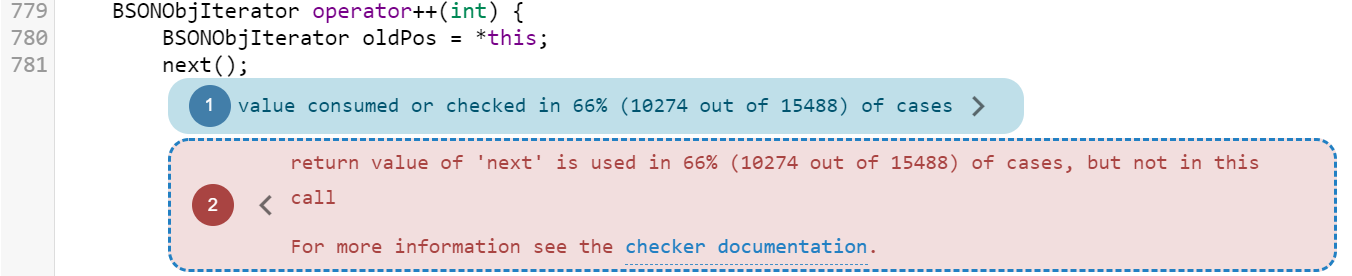
\includegraphics[width=\linewidth]{images/codechecker_first_ss_mongo_multi_50.png}
	\caption{A report of the diagnostics of MongoDB's source on CodeChecker with 50\% threshold and project-level knowledge.}
	\label{fig:mongo50multi}
\end{figure}

We can clearly conclude, that the multipass diagnosis resulted in different warnings. \Cref{fig:mongo50multi}
differs from \cref{fig:mongo50single} in only the percentage, but with a different threshold that could lead to different
results, to either false positives, or false negatives. Our own example, however shows both, since we had a call
that used to give warning when diagnosed separately which with project-level knowledge does not, and one that did not give
any warnings, but now it gives two, because it passed the threshold.

In \cref{lst:motivation-example} we talked about our code getting no warnings without project-level knowledge.
After phases collect and compact, however, the following diagnostics will be emitted:

\begin{listing}[H]
	\begin{minted}{Bash}
	/home/bahramib/MyFolder/TestFolder/b/vec.cpp:7:15:
		warning: return value of 'erase' is used
		in most calls, but not in this one [misc-discarded-return-value]

			c.erase(it);
			  ^

		/home/bahramib/MyFolder/TestFolder/b/vec.cpp:7:15: note:
		value consumed or checked in 66% (2 out of 3) of cases
	\end{minted}
\end{listing}

We can clearly see, that our diagnosis gave us the real results this time.

